\documentclass[11pt,a4paper]{article}

%---------------------------------------------------------
%	Aditional Packages
%--------------------------------------------------------
\usepackage{textpos}
\usepackage{subcaption} % To have multiple plots side by side
\usepackage{float}
\usepackage{url} % enable clickable URLs
\usepackage{listings} % to have code blocks in your document
\usepackage{xcolor}
\usepackage{doi}
\usepackage{microtype}
\usepackage{booktabs}
\usepackage{nicefrac} % creates a fraction that is nicer when used in text \nicefrac{1}{2}

% Define some colors for code 
\definecolor{codegreen}{rgb}{0,0.6,0}
\definecolor{codegray}{rgb}{0.5,0.5,0.5}
\definecolor{codepurple}{rgb}{0.58,0,0.82}
\definecolor{backcolour}{rgb}{0.95,0.95,0.92}

% Defines codeblock styles
\lstdefinestyle{mystyle}{
    backgroundcolor=\color{backcolour},   
    commentstyle=\color{codegreen},
    keywordstyle=\color{magenta},
    numberstyle=\tiny\color{codegray},
    stringstyle=\color{codepurple},
    basicstyle=\ttfamily\footnotesize,
    breakatwhitespace=false,         
    breaklines=true,                 
    captionpos=b,                    
    keepspaces=true,                 
    numbers=left,                    
    numbersep=5pt,                  
    showspaces=false,                
    showstringspaces=false,
    showtabs=false,                  
    tabsize=2
}

% Set the maximum depth sections are counted to and shown in the TOC
\setcounter{secnumdepth}{3} % depth of counting
\setcounter{tocdepth}{3} % depth that toc will show 

% new paragraph style with new line
\newcommand{\myparagraph}[1]{\paragraph{#1}\mbox{}\\}


\lstset{style=mystyle}
\renewcommand{\lstlistingname}{Configuration}% Listing -> Configuration

% Toogle between the two to hide or show images
% \usepackage[draft]{graphicx}
\usepackage{graphicx}
\usepackage[utf8]{inputenc} 
\usepackage{upgreek}
\usepackage{titlesec}
\usepackage{physics} % adds easy derivatives etc. 
%\AtBeginDocument{\RenewCommandCopy\qty\SI} % dont know why
\usepackage{amssymb} % more symbols
\usepackage{amsmath} %enables align environment
\usepackage{multirow}


% \usepackage[showframe]{geometry} % Shows margins in pdf if you want to know what's going on
\usepackage{geometry}
\geometry{
    %a4paper,
	left=40mm,
    % right=20mm,
	top=35mm,
    }

% Use biblatex
\usepackage[backend=biber,
natbib=true,
maxcitenames = 2,
maxbibnames = 5,
minbibnames = 4, 
sorting=none]{biblatex}

\usepackage{csquotes}

\addbibresource{references.bib}
\setlength\bibitemsep{1.5\itemsep}


% --------------------------------------------------------
% CUSTOM STUFF:
\usepackage[textsize=tiny]{todonotes}
\setlength{\marginparwidth}{2cm}
\usepackage{bm}
\usepackage{tikz}
\newcommand{\no}{%
\tikz[scale=0.23] {
    \draw[line width=0.7,line cap=round] (0,0) to [bend left=6] (1,1);
    \draw[line width=0.7,line cap=round] (0.2,0.95) to [bend right=3] (0.8,0.05);
}}
\newcommand{\yes}{%
\tikz[scale=0.23] {
    \draw[line width=0.7,line cap=round] (0.25,0) to [bend left=10] (1,1);
    \draw[line width=0.8,line cap=round] (0,0.35) to [bend right=1] (0.23,0);
}}
\usepackage[table]{xcolor}
%---------------------------------------------------------
\usepackage{hyperref} % enable clickable links to sections, figures, etc. 
\PassOptionsToPackage{unicode}{hyperref}
\PassOptionsToPackage{naturalnames}{hyperref}

% Remove the coloured border around autoref links
\hypersetup{%
pdfborder = {0 0 0}
}



\begin{document}	
\pagestyle{empty}

%---------------------------------------------------------
%	Titlepage
%---------------------------------------------------------

\begin{center}
    \vspace*{1cm}
    \LARGE \bf{Structure recognition with graph neural networks} \\

    \vspace*{2cm}
    \large \bf{An intermediate report for the course "Advanced Projects in Computational Physics 2"}


    \vspace{4cm}
    
    \vspace{1.2cm}
            From\\
            {\bf Stephen Weybrecht} \\
            \today

    \vspace*{6 cm}
    Supervisor: Jonas Buba 
    \vspace*{1 cm}

\end{center}
\clearpage

\begin{abstract}
    The project described in the following lies at the intersection of solid state physics and machine learning. On the one hand there is the physical problem, namely the classification of noisy crystal lattices in 2 and 3 dimensions into their corresponding Bravais lattice group. For this graphs are randomly generated in a first step. These graphs then need to be classified efficiently and robustly, regardless of noise and introduced defects. As is the case with other classification tasks, neural networks promise an interesting approach to this goal and will therefore be the second part of this project. For this special networks designed for handling graph like structures, so called Graph convolutional networks are employed. These use a concept called message passing to efficiently enable graph level classification tasks. \\
    
    By use of these concepts a test accuracy of over 90\% has been achieved for both the 2D and 3D case. Future goals include testing out other features and network architectures for this classification task, as well as the specialisation in defect detection in mono atomic crystal lattices.

    
\end{abstract}
%---------------------------------------------------------
%	Table of Contents
%---------------------------------------------------------
% Generate
\newgeometry{
    %a4paper,
	%left=20mm,
    right=40mm,
	top=35mm,
    } 
\tableofcontents
\restoregeometry
\clearpage
\mbox{}

\pagenumbering{arabic}
\setcounter{page}{1}
 \pagestyle{plain}
%---------------------------------------------------------
%	Report
%---------------------------------------------------------

\section{Theoretical introduction}
\label{sec:Theoretical introduction}

\subsection{Bravais lattices}
\label{ssec:Bravais lattices}
In the first part of the project, our task was to deal with crystal lattices in 2 and 3 dimensions. 
For the following discussion an introduction of the terms "crystal", "basis" and "Bravais lattice" is therefore needed. \\

Following the discussion of \cite{kittelChapter1Crystal2005} an ideal crystal is a periodic, infinite arrangement of atoms in a solid. 
These atoms are arranged in blocks, a so called basis, in a regularly spaced grid, the lattice. 
In other words the lattice represents a schema after which individual atoms or groups of atoms (the basis) are arranged to form the crystal. 
A lattice in $d$ dimensions can be defined by a set of $d$ translation vectors. 
The superposition of integer multiples of these vectors then makes up the lattice \cite{kittelChapter1Crystal2005}. 
In principle the length and direction of these vectors can be arbitrary. 
In this case the lattice would generally not map into itself under translations and rotations -- the lattice is called oblique. 
There are however special sets of translation vectors which form lattices of high symmetry. 
These fundamental lattices are called the Bravais lattices. 
For $d=2$ there are 5 (4 special and one oblique) Bravais lattices, while for $d=3$ there are 14 (13 special cases and one oblique, so called triclinic lattice). 
These are depicted in \autoref{fig:bravais2D} and \autoref{fig:bravais3D} respectively. 

\begin{figure}[htbp]
    \centering
    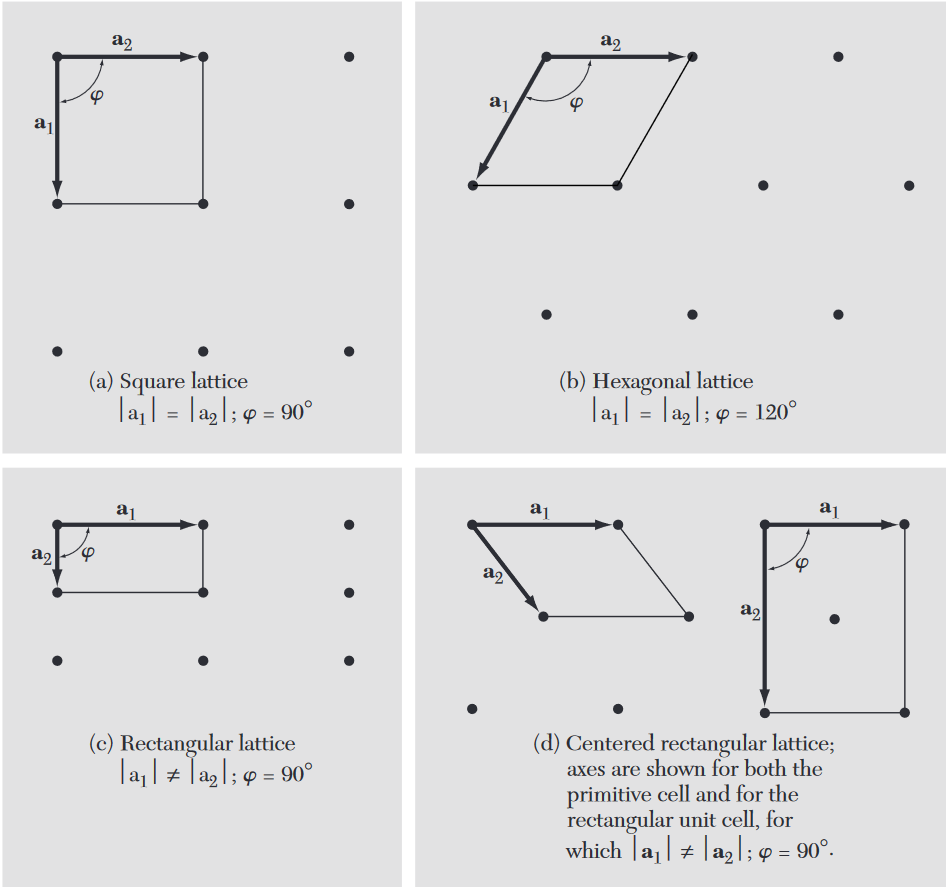
\includegraphics[width=0.6\textwidth]{images/Kittel_7.png}
    \caption{The five Bravais lattices for 2 dimensions. The graphic also illustrates the length of the translation vectors $\bm{a}_i$ and the angle between them in order to make up the corresponding lattice. Taken from \cite[Fig. 7]{kittelChapter1Crystal2005}.}
    \label{fig:bravais2D}
\end{figure}

\begin{figure}[htbp]
    \centering
    \includegraphics[width=0.7\textwidth]{images/Kittel_14.png}
    \caption{The 14 Bravais lattices for the $d=3$ case. 
    One further classifies these lattices into seven types of cells: Cubic ($a{=}b{=}c$, $\alpha {=} \beta {=} \gamma{=}90^\circ$), Tetragonal ($a{=}b {\neq} c$, $\alpha {=} \beta {=} \gamma{=}90^\circ$), Orthorhombic ($\alpha {=} \beta {=} \gamma{=} 90^\circ$), Monoclinic ($\alpha {=} \beta{=}90^\circ {\neq} \gamma$), Triclinic, Triagonal ($a{=}b{=}c$, $\alpha {=} \beta {=} \gamma <120^\circ {\neq} 90^\circ$), Hexagonal ($a{=}b{\neq} c$, $\alpha {=} \beta{=} 90^\circ, \gamma{=} 120^\circ$). 
    Note that in the prior notation $a$, $b$ and $c$ denote the lengths of the translation vectors, $\alpha$, $\beta$, $\gamma$ the angles between them and omitted length or angle relations mean they can be arbitrary. 
    These groups are again subclassified based on their lattice structure into simple "P", body-centred "I", base-centred "C", face-centred "F". 
    As mentioned, all lattices are special cases of the general, triclinic case. The graphic is taken from \cite[Fig. 14]{kittelChapter1Crystal1971}.}
    \label{fig:bravais3D}
\end{figure}


\subsection{Basics of Machine Learning}
\label{ssec:BAsics of Machine Learning}
In the following the basic principles behind Artificial Neural Networks (NNs) and Machine Learning will be explained. 
This chapter follows closely the discussion in \cite{kubatChapter5Artificial2017}, the upcoming equations and concepts are therefore taken from this source. 
For this introduction the simplest model will be used as an example to explain the key concepts, as a generalisation to more sophisticated models is straightforward once the basic principles are understood. 
This simple model is the so called Perceptron, a network consisting of fully connected units, so called neurons, aranged in layers. 
This NN consists at least of an in- and output layer which are usually supplemented by one or more hidden layers in between. 
A neuron $j$ in layer $l$ has as its attribute a feature vector $x^{(l)}_j$ and each connection is associated by a weight $w_{ij}^{(l-1)}$ where this weight represents the connection between neuron $i$ in layer $l-1$ to neuron $j$ in layer $l$. 
The general idea is that each neuron takes as input the "signals" from every neuron it is connected to in the previous layer (ie. in our example of a fully connected network the signals from every neuron in the prior layer) and updates its own value according to the fololowing weighted sum:
\begin{equation}
    \label{eq:NN weighted sum}
    x^{(l)}_j = f\left(\sum_i w_{ij}^{(l-1)} \cdot x^{(l-1)}_i + b^{(l-1)}\right)
\end{equation}
Here the weighted sum is further modified by a layer dependent bias vector $ b^{(l-1)}$. 
Furthermore the aggregated "signal" is usually modified by an non-linear activation function $f$. 
Using the above update rule it is now clear, that a forward pass through the model can be accomplished by suppliing an input vector $x^{(1)}_i$ and using \autoref{eq:NN weighted sum} iteratively to achieve an output at the final layer $n$ $x^{(n)}_i$. \\

In this simple supervised training example each input vector $x^{(1)}_i$ is acommpined by a target vector $t_i$ which is the wanted output of the network, given said input vector. 
For training one must now specify a so called loss function, which represents how far the output of the NN deviates from said target (e.g. the mean squared difference between them). 
It is apparent that the goal of training must be to minimize said loss. 
This is done via so called gradient descent where the gradients of the loss function with respect to the model parameters $w_{ij}^{(l-1)}$ and  $ b^{(l-1)}$ is calculated. 
In the parameter space of these weights and biasses this gradient points toward regions where the loss changes the most. 
In the process of backpropagation the NN parameters are now updated using these gradients. 
The algorithm goes backwards through the network (From layer $n$ to $1$) and updates the paramaters using calculated gradients such that the loss is minimized. 
The magnitude of this update is influenced by the Learning rate $\eta$ which is an important hyperparameter that needs to be set for training. 
How this update works in detail goes beyond the scope of this introduction, further details can for example be found in \cite{kubatChapter5Artificial2017}. 
Once this training is completed for all input training samples one epoch of training has been completed. 
Usually the training of a NN is repeated for many epochs. \\

Lastly, once the training was deemed sufficient, one used a different, so called validation dataset, which was not used during training to asess the final performance metric of the model. 

\subsection{Graph neural networks}
\label{ssec:Graph neural networks}
The lattices as discussed in the prior section are a collection of atoms linked by bonds and can therefore be suitably represented by a graph, consisting of nodes and edges. 
If we want to apply machine learning to crystal lattices, we therefore need models that are well suited for data organized in a graph-like manner. 
What follows is a basic introduction to such networks, specifically graph convolutional neural networks (GCNs). \\

GCNs take inspiration in the already well-established convolutional neural networks in which a typical layer consists of a trainable kernel that can be applied on ordered, grid-like training data of arbitrary size and shape (e.g.. images) \cite{khemaniReviewGraphNeural2024}. 
GCNs represent a generalisation of this concept onto unordered nodes with a variable number of neighbours. 
Each GCN-layer uses so called message passing in order to update the node state $h^{(t)}_u$ of a time $t$ to the next step $h^{(t+1)}_u$ as shown in \autoref{eq:messagepassing} \cite[eq. 4.1]{khemaniReviewGraphNeural2024}.
\begin{equation}
    h^{(t+1)}_u = UPDATE^{(t)}\left(h^{(t)}_u, AGGREGATE^{(t)}\left(\left\{h^{(t)}_v, \forall v \in N(u)\right\}\right)\right)
    \label{eq:messagepassing}
\end{equation}
In the above equation $UPDATE^{(t)}$ and $AGGREGATE^{(t)}$ could be any differentiable functions i.e. also neural networks, and $N(u)$ denotes the neighbourhood of $u$ meaning all directly connected nodes in the graph. 
This equation implies the following update schema that is also depicted in \autoref{fig:messagepasisng}: \\
The starting point is a graph, consisting of nodes with feature vectors and connections, that could also have features. 
For each node, messages from neighbouring nodes are aggregated to a single message by taking a weighted mean of the neighbouring nodes feature vectors. 
This operation can also be weighted by use of edge features. 
This message is then passed to a non-linear update function (e.g.. ReLU), that updates the node in question for the next time step. 
After the update is completed, further operations can be performed depending on the wanted classification scheme. 
In the following graph classification is used, which means all feature vectors are pooled in a last step, in order to get a single quantity that is descriptive of the entire graph \cite{khemaniReviewGraphNeural2024}.
\begin{figure}[htbp]
    \centering
    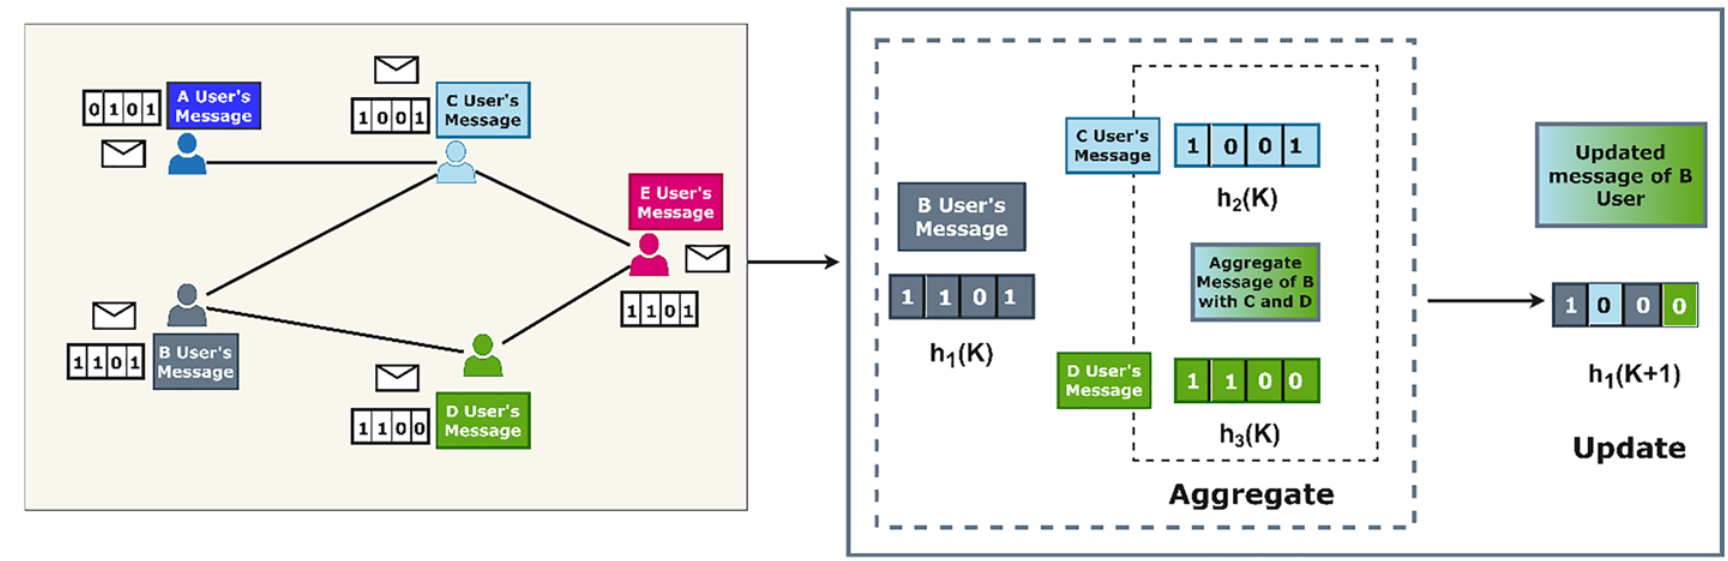
\includegraphics[width=0.9\textwidth]{images/khemani7.png}
    \caption{A graphic representation of the update schema for message passing graph neural networks. Taken from \cite[Fig. 7]{khemaniReviewGraphNeural2024}.}
    \label{fig:messagepasisng}
\end{figure}


\section{Results}
\label{sec:Results}
In the following I will give a chronological overview of the topics I worked on during this project. 
This started with the generation of training data, namely Bravais lattices in two and three dimesions. After this I worked on Bravais lattice classification of noisy and defective lattices to gain familiarity with the GNN architecture and a Machine Learning library. Lastly I worked on defect detection using Graph Autoencoders. 

\subsection{Generation of Training data}
\label{ssec:Generation of training data}
As a first step Bravais lattices in two dimensions (2D) and three dimensions (3D) needed to be created. 
For this ideal Bravais lattices with roughly a unit spacing between nodes are created in a first step. 
Additionally random Gaussian noise is added. 
For further variety in training samples, graphs are additionally scaled by random constants to provide non-uniform node-spacing within one Bravais lattice group. 
At this step different kids of defects are introduced. 
These defects either are a removal of randomly many nodes at random positions or the addition of a single, randomly placed node within the lattice. 
What kind of process has been used will be explained in detail in the following sections, as it is dependent on the task at hand. 
After the nodes have been placed, noise was added and defects were introduced, the connections between nodes are determined by searching for the neighbours within a given radius (that also depends on the noise amplitude) and connecting all nodes, that lie within said radius. 
By these means the random noise and defects are also included within the structure of the graph and have an influence in message passing. \\

The features used depend on the task of the GNN -- either graph classification into one of the Bravais lattice groups or defect detection. 
In the following a in-depth overview over all different features used is given such that the later sections can focus on the Neural Network part. \\
As edge features a selection of the following was used: 
\begin{itemize}
    \item The 2D or 3D connection vectors between nodes
    \item Their respective length
\end{itemize}
The node features tested are the following:
\begin{itemize}
    \item The amount of nearest neighbors i.e. the count of connected nodes
    \item The bond orientational order parameter (BOO)\\
    As the name suggests the BOO quantifies the "order" of the bonds around a node. 
    It can be computed for different orders $l$ and can be used to differenciate between different crystal sructures by quantifying their $l$-fold symmetry, see e.g. \cite{steinhardtBondorientationalOrderLiquids1983}. 
    Importantly symmetry is broken near defects, which is why the BOO seems a promising node feature for defect detection. 
    In 2D the BOO of node $j$ and order $l$ is given by
    \begin{equation}
        \label{eq:boo2d}
        \mathrm{BOO^{2D}}_j = \left|\frac{1}{N} \sum_k \mathrm{exp}(il\theta_{jk}) \right|^2
    \end{equation}
    Where we sum over all $N$ neighbors $k$ of node $j$ and $\theta_{jk}$ represents the angle of the $j$-$k$-connection with resprect to some reference direction. \\
    In 3D I used one of the rotational invariants defined as 
    \begin{equation}
        \mathrm{BOO^{3D}}_j = \sqrt{\frac{4\pi}{2l+1} \sum_{m=-l}^{l} \left| \frac{1}{N} \sum_k Y_{lm}\right|^2}
    \end{equation} 
    Here the sum ranges again over all neighbors $k$ and adds the spherical harmonics $Y_{lm}$ dependent on the given order of the BOO and the angles between nodes $j$ and $k$ and an arbitrary refrence direction. 
    \todo{CITATIONS}
    As symmetry is also broken at the edges of the generated graphs, for the calculation I take care to apply sufficient padding of extra nodes around the graph (which are later removed) in order to mitigate edge effects. 
\end{itemize}

\subsection{Bravais lattice classification}
\label{ssec:Bravais lattice classification}

\subsection{Defect detection}
\label{ssec:Defect detection}
\subsubsection{Introduction}
The next goal was to build a GNN tasked with defect detection in 2D and 3D lattices. 
As this has proven itself quite hard with the Dominant network I will introduce in the following the present chapter will give an overview over the things I investigated rather than straight-forwardly presenting a positive result. 
For this the general setup and network architecture is explained in a first step, after which all different tests will be explained. 
At the end I will discuss possible reasons for the bad performance of the Dominant network and suggest network architectures that are possibly better suited for this task. 
It should also be remarked that I will focus the following discussion on 2D graphs, firstly because of time constraints due to the extensive tests I needed to do, secondly because it is not helpful or illustrative to investigate more complex and worse visualisable 3D graphs when even the simple 2D cases show bad performance. \\

Data was generated as described in \autoref{ssec:Generation of training data}. 
As I investigated different feature combinations, the exact features used will be shown for each test specifially. 
Features were taken out of the feature pool shown in \autoref{ssec:Generation of training data}. 
Per graph one defect was added by adding an additional node at a random position. 
This defect node is different than the others both on a structural level (higher connectivity than the rest of the graph) but also on an attribute level (it breaks symmetry which has influence on the BOO, additionally, on average, the lenght of connected edges is smaller and the number of neighbors higher). \\

I looked at many different network setups, layers and features and therefore needed to keep the training time in a reasonable scope which is why I chose to use 250 graphs for each of the 5 Bravais lattice types. 
This resulted in a total of 1250 graphs, of which 1000 were used for training and 250 for validation. 
Each network/feature combination test consisted of training the network over 50 epochs and averaging the results over five different random network initialisations in order to achieve good convergence of the loss-curves and a statistically more meaningful result. 
For all of the following tests a batchsize of 16 and the Adam optimizer were used. 
The learning rate was set to 0.001 if not stated differently. 
If the test used edge features GINEConv layers \cite{pygteamGINEConv2024} were used for the construction of the encoder and attribute decoder, else GCNConv layers \cite{pygteamGCNConv2025} were used.
As activation functions and the number of neurons and layers were varied, they will be stated when talking about the specific test performed. \\

\subsubsection{The Dominant Architecture}
I was tasked to implement the Dominant network as described in \cite{dingDeepAnomalyDetection2019}. 
This network uses a Graph Autoencoder i.e. an Autoencoder consisting of Message passing layers to handle graphs. 
Autoencoders are a special kind of neural networks that utilise unsupervised training. 
The goal of this type of network is to reconstruct an the input data as best as possible. 
This task would be trivial if it were not for an important feature of autoencoders: 
The hidden layers reduce in dimensionality until a minimum number of trainable parameters is reached at the so called bottleneck after which the dimensionality again increases until the input dimensionality. 
It is expected that this compression and de-compression works better for large scale recurring structures (e.g. a periodic arrangement of nodes) then for outliers (e.g. the defect node) which makes this approach promising for the task at hand \cite{dingDeepAnomalyDetection2019}. 
A sketch of the structure of the Dominant network is shown in \autoref{fig:Dominant}.
\begin{figure}[htbp]
    \centering
    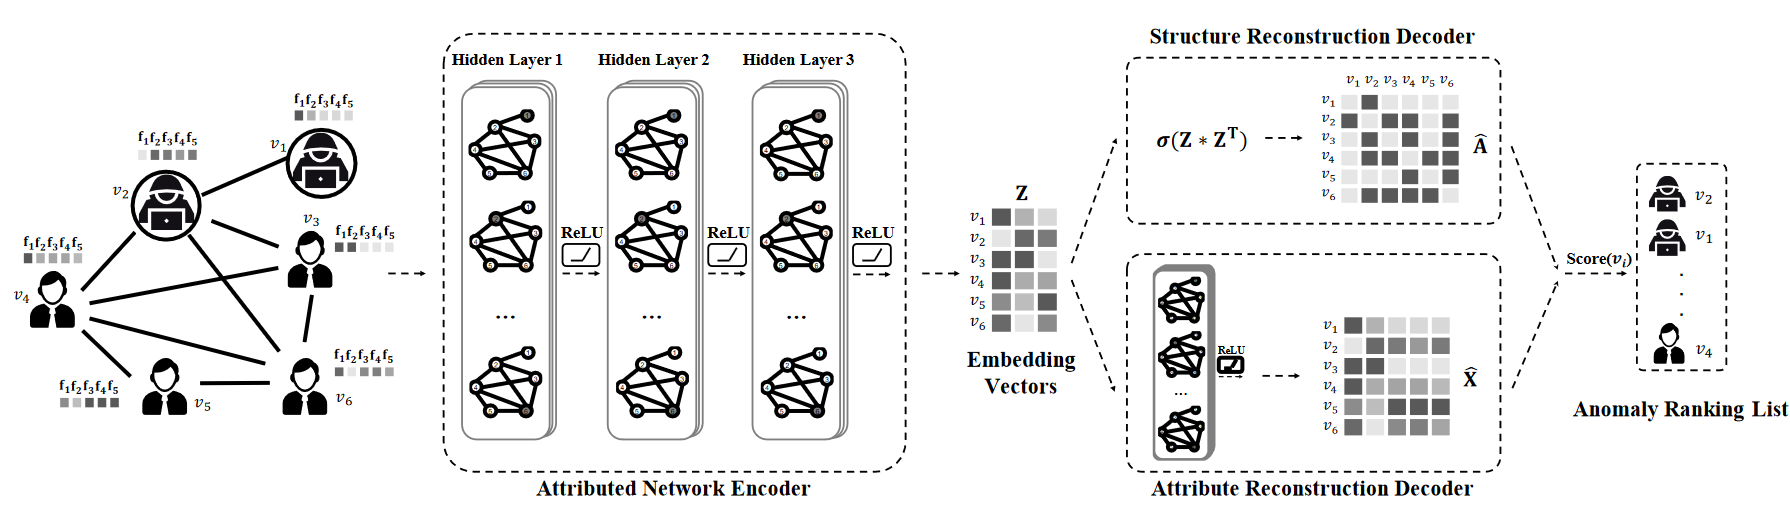
\includegraphics[width=0.8\textwidth]{images/ding_1.png}
    \caption{A sketch of the structure of the Dominant network is shown. The shown number of layers and activation functions do not necesarrily reflect the ones used in the following, as different test have been performed. Taken from \cite[Fig.1]{dingDeepAnomalyDetection2019}}
    \label{fig:Dominant}
\end{figure}
A training set of graphs with outliers is first input into the encoder. 
This encoder consists of message passing layers that reduce in feature dimensionality until the bottleneck is reached. 
The graph data is maximally compressed into a so called embedding vector $z$. 
This is then decoded in two different decoders: 
The structure reconstruction decoder aims to reproduce the input adjacency matrix, which is a possible reprensentation of the edges and their features in a graph. 
This is done by calculating the matrix product of the column vector $z$ with the row vector $z^T$ leading to a matrix of shape $N\cross N$ where $N$ is the number of nodes. 
This can be interpreted as an adjacency matrix. 
Furthermore a non-linear activation function (like a sigmoid) can be applied.  
Additionally the attribute reconstruction decoder aims to reproduce the nodal features of the input graph. 
This is done by use of an additional GNN which increases in feature dimensionality. 
In the following I choose the encoder and decoder network symmetrically. 
After getting both reconstructions a loss can be calculated (this is not shown in \autoref{fig:Dominant}) with which the model is trained \cite{dingDeepAnomalyDetection2019}:
\begin{equation}
    \label{eq:dominant loss}
    \mathcal{L} = (1-\alpha) \left\lVert A-\hat{A} \right\rVert _F + \alpha  \left\lVert X-\hat{X} \right\rVert _F
\end{equation}
Here $\alpha$ is a fixed hyperparamter weighting the attribute versus the reconstruction loss, $A$ and $\hat{A}$ are the input and reconstructed adjacency matrices, $X$ and $\hat{X}$ the input and recostructed node feature matrices and the symbol $\left\lVert\cdot  \right\rVert _F$ represents the Frobenius norm. 
Note that compared to \cite{dingDeepAnomalyDetection2019} I have omitted squaring the norms as this would have lead to extremely large losses which would have needed additional normalisation to achieve a good convergence without offering any benefit. 

Once training is deemed sufficient, a final anomaly score can be calculated for each node $i$ to evalute the model \cite{dingDeepAnomalyDetection2019}:
\begin{equation}
    \label{eq:dominant score}
    \mathcal{S}_i = (1-\alpha) \left\lVert a_i-\hat{a_i} \right\rVert _2 + \alpha  \left\lVert x_i-\hat{x_i} \right\rVert _2
\end{equation}
Here $a_i$, $\hat{a}_i$, $x_i$, $\hat{x}_i$ represent the rows of the matrices $A$, $\hat{A}$, $X$, $\hat{X}$ resprectively and $\left\lVert\cdot  \right\rVert _2$ represents the usual vector 2-norm. 
Note that while \autoref{eq:dominant loss} and \autoref{eq:dominant score} look rather similar, they are not quite the same. 
The loss function copmputes a single scalar loss for each input graph and is used during training. 
The score function computes one scalar anomaly score for each node in the graph and is only used for the defect prediction at the end, as larger anomaly scores represent a higher probability of the node beeing an outlier. 
\todo{how final score}

\subsubsection{Results}
I performed multiple tests with differently structured layers, activation functions, learning rates $\eta$, loss weight $\alpha$, dropout and data paramters. 
These I will present in the following to show, that no matter the chosen hyperparamters the training and performance of the NN is bad. 
In a first step $\eta$ and the use of dropout was varied, after which the best features, network structure, activation functions and $\alpha$ were explored in subsequent tests. 
When varying one or two related parameters the others were kept fixed. 
All hyperparameters for the different tests A-E are tabularised in \autoref{tab:hyperparameters defect detection} for referencing them in \autoref{label} \todo{figures}. 

\begin{table}[htbp]
    \centering
    \begin{tabular}{c|c|c|c|c|c|c|c|c|c}
        test & layers & structure & A-act. & S-act. & $\eta$ & DO & $\alpha$ & NN & BOO \\\hline\hline
        A1 & GINE & 6432 & $\sigma$ & ReLu & 0.001 & \no & 0.5 & \yes & \yes \\\hline
        A2 & - & - & - & - & 0.005  & -  & - & - & - \\\hline
        A3 & - & - & - & - & 0.01   & -  & - & - & - \\\hline
        A4 & - & - & - & - & 0.0005 & \yes & - & - & - \\\hline
        A5 & - & - & - & - & \cellcolor{black!20} 0.001  & \cellcolor{black!20} \yes & - & - & - \\\hline
        A6 & - & - & - & - & 0.003  & - & - & - & - \\\hline
        A7 & - & - & - & - & 0.005  & - & - & - & - \\\hline
        A8 & - & - & - & - & 0.01   & - & - & - & - \\\hline\hline
        B1 & GINE & 6432 & $\sigma$ & ReLu & 0.001 & \yes & 0.5 & \cellcolor{black!20}\yes & \cellcolor{black!20}\yes \\\hline
        B2 & - & - & - & - & - & - & - & \no & \yes \\\hline
        B3 & - & - & - & - & - & - & - & \no & no $l=2$ \\\hline\hline
        C1 & GCN & 6432  &  ReLu & ReLu & 0.001 & \yes & 0.5 & \yes & \yes \\\hline
        C2 & - & 6543  &   -   &  -   &   -   &  -   &  -  &  -   &  -   \\\hline
        C3 & \cellcolor{black!20}GCN &\cellcolor{black!20} 6531  &   -   &  -   &   -   &  -   &  -  &  -   &  -   \\\hline
        C4 & - & 65432 &   -   &  -   &   -   &  -   &  -  &  -   &  -   \\\hline
        C5 & GINE& 6432  &$\sigma$& ReLu & 0.001 & \yes & 0.5 & \yes & \yes \\\hline
        C6 & -& 6543  &   -   &  -   &   -   &  -   &  -  &  -   &  -   \\\hline
        C7 & -& 6531  &   -   &  -   &   -   &  -   &  -  &  -   &  -   \\\hline
        C8 & -& 65432 &   -   &  -   &   -   &  -   &  -  &  -   &  -   \\\hline\hline
        D1 & GCN & 6432 &$\sigma$&$\sigma$& 0.001 & \yes & 0.5 & \yes & \yes \\\hline
        D2 &  -  &  -   &$\sigma$& none  &   -   &  -   &  -  &  -   &  -   \\\hline
        D3 &  -  &  -   &\cellcolor{black!20}  ReLu  & \cellcolor{black!20} ReLu  &   -   &  -   &  -  &  -   &  -   \\\hline
        D4 &  -  &  -   & ReLu  & none  &   -   &  -   &  -  &  -   &  -   \\\hline
        D5 &  -  &  -   & ReLu  &$\sigma$&   -   &  -   &  -  &  -   &  -   \\\hline\hline
        E1 & GCN & 6432 & ReLu & ReLu & 0.001 & \yes & 0.3 & \yes & \yes \\\hline
        E2 &  -  &  -   &  -   &  -   &   -   &   -  &\cellcolor{black!20} 0.4 &   -  & -    \\\hline
        E3 &  -  &  -   &  -   &  -   &   -   &   -  & 0.5 &   -  & -    \\\hline
        E4 &  -  &  -   &  -   &  -   &   -   &   -  & 0.6 &   -  & -    \\\hline
        E5 &  -  &  -   &  -   &  -   &   -   &   -  & 0.7 &   -  & -    \\\hline\hline
    \end{tabular}
    \caption{Listed are the used hyperparamters for each test A-E. Each row corresponds to one network/data-comnbination that was used for training 5 times 50 epochs which were then averaged to produce the curves in . "-" means the parameter is the same as in the row above. Cells with grey background indicate the best results of each test. The columns represent from left to right: The used layer (either GINEConv or GCNConv), the dimensionality of the encoder layers with mirrored decoder (e.g. 6432 means the input node feature vector of dimension 6 is reduced to a hidden feature vector of dimension 4 in the first, 3 in the second hidden layer and 2 in the bottleneck), the attribute (A-act.) and structure (S-act.) decoder activation function, the learning rate, whether a dropout with probability 0.5 was used, the loss weighting, whether the number of nearest neighbors (NN) or the bond orientational order parameter (BOO) have been used as features.}
    \label{tab:hyperparameters defect detection}
\end{table}
\todo{refs}
\todo{check alpha 0.4 or 0.3}

As mentioned in a first test the influence of the learning rate $\eta$ and the use of dropout were examined. 
To make matters easier a dropout with fixed probability of 0.5 has been applied between each layer during training. 
For evaluation this dropout is automatically switched off. 
For this first test it seemed best to supply the entwork with maximal information, which is why all node features (BOO of order $l=2,4,6,8,10$ and the number of neighbors) were used as well as the length of edges as edge features. 
Because edge features are used, GINEConv layers are employed (They support edge features in contrast to GCNConv) in a structure of 6432, meaning the input vector dimensinality is reduced from 6 to 4 to 3 to 2 in the encoder and increased again symmetrically in the attribute decoder. 
As activation a sigmoid was used after each hidden layer for the attribute reconstruction (taking care not to apply a sigmoid to the oputput) and a ReLu function was used for the structure decoder (which seemed sensible as the adjacency matrix can have values bigger then 1 because of the edge features). 
All these choices are also listed in \autoref{tab:hyperparameters defect detection} and will therefore be discussed less extensive for the following tests. 
Now the network was run for larger and smaller $\eta$ in combination with dropout or without dropout for 5 times 50 epochs. 
Each training epoch the network was evaluated by calculating its loss and detection score based on a test sample that was not used prior in training.
These curves are then averaged over the mentioned 5 random network initialisations to get a more robust and comparable result, as single runs have proven themselfes to be very dependent of initalisation. 
The results are shown in \autoref{fig:defect detection A}, where one can see that the network performes best, if dropout and $\eta=0.001$ is implemented. 
\begin{figure}[htbp]
    \centering
    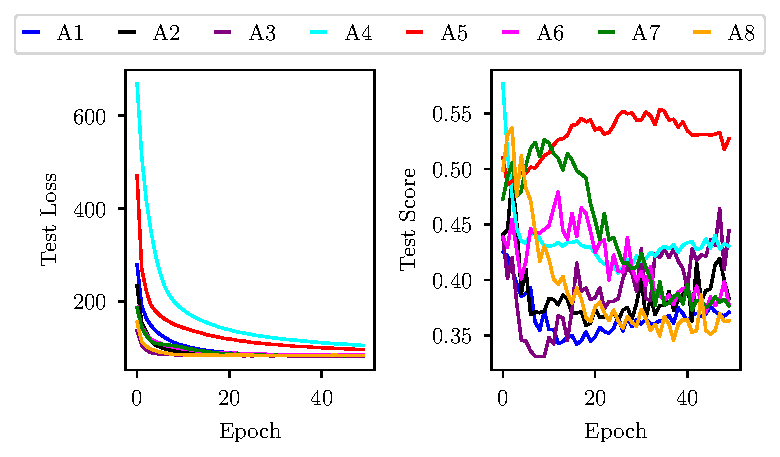
\includegraphics{images/plots/defect_detection_A.pdf}
    \caption{Shown are the test results for Test A. For a listing of hyperparamters see \autoref{tab:hyperparameters defect detection}.}
    \label{fig:defect detection A}
\end{figure}
However, the central problem that will alos govern the tests shown in the following also becomes apparent. 
While the loss is minimized quite well by the network and a stable loss is reached after around 50 epochs indicating the network has trained all it can given the input network and data parameters, the score behaves quite differently. 
Namely there are two problems. 
First of all it is immediately apparent that the score does not increase steadily with falling loss. 
Rather it increases and decreases seemingly at random even for the "optimal" parameter choice shown in red. 
\todo{is the score statistically compatible with a random walk?}
Secondly one can see the score already starts on quite a high level of roughly 50\% correct guesses. 
As the score is determined by the percentage of test graphs where the true anomalous node is within the top five highest anamoly scores however and there are roughly 100 nodes in each graph the initial score should be much lower if the network would just perform a random guess. 
This indicates the network in its untrained state is in fact not performing random guesses but rather there is a systematic component "pushing" the network towards the right guess even when all weights are initialised randomly. 
I reason this follows from the nature of how the anomolous node affects the graph and therefore also the network structure. 
Firstly a spurous node increases connectivity around it as it increases local density and with that the amount of connected nodes as they are determined by connecting all nodes within a said radius. 
In the message passing layers this highly connected node now receives more messages that are also different from those other more regular nodes receive. 
The number of neighbors for instance is higher on average, while the edge length is lower and the BOO also differs in all orders. 
I assume that this increases the mean squared reconstruction error of this node on average even for a random initialisation and therefore leads to a slightly higher anomaly score in a local neighborhood around the anomolous node. 
This in turn leads to the fact that the network has quite well performance from the start. \\

What I want to stress however is that this high score is not a good thing. 
It just stems from systematics that indicate that a machine learning approach with this architecture is not well suited for defect detection as learning is the facto not needed. 
This further indicates that there might be a simpler algorithm that uses a structure similar to the dominant network but can work completely without training just from the connectivity and feature space of the graph itself. 




\section{Results so far}
\label{sec:Results so far}
\todo{ Wie groß war der Datensatz? Wie wurde er aufgeteilt für
Training/Validation}
\todo{Wie lief der Trainingsprozess ab? (Optimizer, batchsize, learning
rate etc., gerne loss/accuracy plotten)}
\todo{ * Verwendete Layer und Aufbau des Netzes beschreiben (welche Methode
wurde für das Pooling verwendet? wie kommen wir vom Pooling zu
unserer Wahrscheinlichkeitsverteilung der Gittertypen?)}
The main tasks so far were to gain familiarity with a machine learning Python library by working on graph classification of 2- and 3-dimensional Bravais lattices. 
For this I chose PyTorch, as it has a library for working with graph neural networks called PyTorch Geometric (PyG) built on top of it. 
The first step for both cases was to generate the training data. 
For this ideal Bravais lattices were created in a first step, to which random (Gaussian) noise, and defects (meaning a removal of a random number of nodes at random positions) were added. 
For further variety in training samples, graphs were additionally scaled by random constants to provide non-uniform node-spacing within one Bravais lattice group. 
After the nodes have been placed and noise was added, the connections between nodes are determined by searching for the neighbours within a given radius (that also depends on the noise amplitude) and connecting all nodes, that lie within said radius. 
By these means the random noise and defects are also included within the structure of the graph and have an influence in message passing. \\
The size of the graphs have been chosen as follows. 
For the plane lattices a size of 10 by 10 nodes has been chosen in order to give the network enough information about each training sample to learn something about the Bravais lattice. 
For the 3D lattices a  size of 10 by 10 by 10 nodes has been tried but deemed unpractical as the time effort for training is quite large. 
This in turn leads to only being able to use a low number of training samples which leads to low accuracies of around 60\%. 
A better approach proved to be using graphs of size 5 by 5 by 5 nodes which cuts the total number of nodes per graph by a factor of 8 while still giving the network enough information to determine the lattice correctly. \\
For node features the number of neighbouring nodes has been chosen while each edge has the (two or three dimensional) connection vector between its corresponding nodes as its feature. 
This has proven itself to be enough information to classify a test dataset of random graphs with more than 90\% accuracy for both cases. 
For classification each lattice was labeled by its one-hot encoded type that was then compared by using the  cross entropy loss function during training. 
As connection vectors carry quite a lot of information, for future tests other features like connection lengths or binding angles are planned in order to see, how much information about the lattice is needed to suitably classify it. 
For these preliminary results a high degree of information in the features and shallow neural network (2D: 2 GINEConv layers \cite{pygteamGINEConv2024} with a total of 12 hidden neurons, 3D 3 GINEConv layers with 50 hidden neurons total) was however used as a proof of concept and to see whether graph generation worked. 



\section{Plans for the future}
\label{sec:Plans for the future}
In the following the goals for the remaining part of the project will be discussed and a rough time estimate for each step will be given. 
As graph generation and classification has worked rather well so far, I expect only little changes to be made to the already existing code. 
Further things to improve or try out with the existing method are varying node and edge features and choosing different layers or a different network structure. 
By this investigation one could find out the minimal amount of information the network needs to classify Bravais lattices and the most efficient network architecture. 
As the tasks discussed so far however only served as a kind of general introduction into the actual topic that is specific to me, extensive experiments with the old goal of lattice classification are not planned. 
Instead the focus shifts towards a new goal, namely the detection of defects in mono atomic crystals. 
I expect to be able to reuse significant parts of the lattice generation code I have written so far, although significant changes in the network architecture and features will most likely be made. 
A meeting with Jonas Buba for discussing the specifics for the future project is scheduled for Wednesday, the 11.12. 
After that I plan to finish the remaining experiments having to do with the old goal of Bravais lattice classification until the end of December. 
During the same time I want to gain familiarity with the theory and suitable approaches for defect detection by reading literature and starting to code. 
Until the mid of January I plan to finalise the coding part of the project, to be able to focus on writing the report and preparing the final presentation during the remaining time. 

\section{Code availability}
\label{sec:Code availability}
The code written for this project is made available in the following Git repository: \url{https://github.com/SteWey0/Computerpraktikum/}

%---------------------------------------------------------
%	Bibliography
%---------------------------------------------------------

\newgeometry{
	%a4paper,
	left=40mm,
    % right=20mm,
	top=35mm,
}
\renewcommand\refname{Bibliography}
% \printbibliography
\printbibliography[
heading=bibintoc,
title={Bibliography}
]


\end{document}